The first research questions where I did research to find the optimal pool size for the fixity information had two different approaches, the first was to minimize the cost and the second was to maximize the efficiency. The two of them were inversely correlated, where to minimize the cost the pool size was actually N, since there was only one writing transaction on the blockchain when we have only one pool on ingest. On the other hand, a pool size of N is extremely inefficient on retrieval, where I have to replace the whole ingest bulk with fresh copies if only one object in the pool is corrupt, since I cannot determine any more which object in the pool got corrupted due to the nature of hash lists. Therefore, I had to also account the number of data scrubbing operations into the optimal pool size, resulting in Equation \ref{eq:expected_data-scrubbing}. The pool size is therefore heavily dependent on the prevalence of corruption in the ingest bulk, where if the prevalence is high smaller pool sizes are favorable. The goal of this thesis was to reduce the cost of the fixity storage by at least 50\%, this goal can be met when the optimal pool size is at least two, which is guaranteed with a prevalence lower than 35.9\%, as seen in Figure \ref{fig:threshhold}.
\begin{figure}[h]
    \caption{For a prevalence of corruption of maximum 35.9\%, an optimal pool size of at least two is guaranteed}
    \label{fig:threshhold}
    \centering
    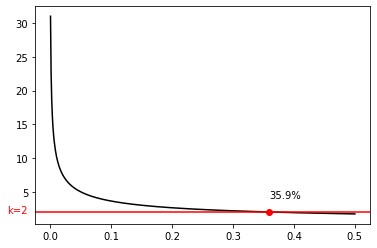
\includegraphics[width=0.5\textwidth]{threshhold.png}
\end{figure}
What happens if the prevalence is higher than 35.9\%, the optimal pool size would be between 1.0 and 2.0 which is not practical since a pool can not include 1.42 objects, therefore I have decided to round the result up from Equation \ref{eq:poolsize} which results in Figure \ref{fig:threshhold-ceil}.
\begin{figure}[h]
    \caption{For a prevalence of corruption of maximum 35.9\%, an optimal pool size of at least two is guaranteed}
    \label{fig:threshhold-ceil}
    \centering
    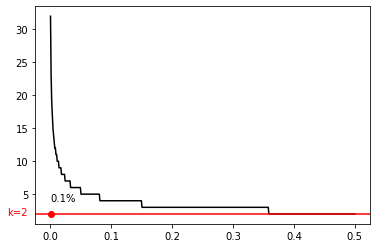
\includegraphics[width=0.5\textwidth]{threshhold-ceil.png}
\end{figure}
For the second research question, I have compared two different approaches for pooled testing. Where the efficiency of both strategies is compared to the efficiency of individual testing. The efficiency of individual testing for sample population of 100 objects where 20 of them are corrupt, meaning that I need 100 writing  + 20 scrubbing operations during the preservation process. With two stage hierarchical pooling an efficiency of 2.24 can be achieved, meaning that this strategy is more than two times as efficient as individual testing. In the format-corpus dataset there were just a few file extensions of 90 that were altered and had a prevalence of corruption greater than 0.0, suggesting that the two-stage strategy was not optimal, since non-volatile files would give been grouped together creating unnecessary traffic on repairing a corrupt pool. Therefore, I have proposed a context-sensitive approach where the inner group prevalence of each file extension is taken into account. Each group in the ingest-bulk is assigned to an own pool with their respective pool size. For instance, in table \ref{tb:efficiency} the file extension PDF has 8 corrupted objects out of 106, which results in a pool size of 8, whereas the XML extension has a much higher corruption rate with an optimal poolside of 2. The context-sensitive approach takes these differences into account and pools homogenous groups, where groups with 0.0 prevalence of corruption can be grouped with a pool size as large as the inner group. With this method, groups with low prevalence can be pooled with large poolside and therefore reduce the cost and increase the efficiency even more than individual testing or two-stage hierarchical pooling.
The third research question had a surprising result, given that metadata has a much higher prevalence of corruption rate than the object themselves, two-stage hierarchical pooling increases its efficiency with split off metadata whereas the context-sensitive strategy looses efficiency by a large margin. This is due, the double amount of objects needed to be processed during the preservation process where the context-sensitive approach can not make up for it, whereas the two-stage hierarchical approach is able to increase the efficiency: due to the low average prevalence of corruption. Because I have N/2 objects with very high prevalence but with the same file extension, therefore we have only one inner group in the dataset with e.g. p=0.99 where the N-1 file extensions have a very low prevalence rate. The imbalance of alteration rates, see Table \ref{tb:context-sensitive}, is favorable because the average prevalence rate gets very low which results in a large pool size in the two-stage approach.
The limitations of the strategies proposed in this thesis is the missing data on prevalence rates on digital objects, this is due to the fact that I would have had to monitor an archive and measure the amount of times an object has changed. In this thesis, I have arbitrarily chosen prevalence rates for the objects and their metadata, see Table \ref{tb:split-off}. Future work may propose a method on how to estimate the prevalence rate of an ingest-bulk in order to calculate the real optimal pool size for the bulk.
The results indicate that the cost for the decentralized fixity storage can be reduced, depending on the prevalence rate of the digital objects by at least 50\%, given that the optimal pool size for an ingest-bulk is at least 2.